%% muonDetectionSystem.tex
%%

%% ==============
\chapter{Muon detection system}
\label{ch:The muon detection system}
%% ============== 
  The need for low background rates at the FPD requires for a good knowledge of background sources. Despite magnetic reflection and wire electrodes described in chapter \ref{ch:The KATRIN experiment:sec:Experimental setup:subsec:BackgroundSources}, cosmic ray and particularly cosmic muon induced background may be an issue for the KATRIN experiment. To gather and assess muon related data, a muon detection system has been designed and set up at both the monitor spectrometer and the main spectrometer. Both are built on the same principle. Scintillator panels (sec. \ref{ch:The muon detection system:sec:Scintillator modules}) are permeated by muons causing photon emissions in the material. The photons are detected by photomultipliers (sec. \ref{ch:The muon detection system:sec:Photomultipliers}) and converted to detectable electrical signals. Readout is handled by a data acquisition crate ``DAQ'' (sec. \ref{ch:The muon detection system: sec: DAQ}) that is controlled via the Object-oriented Real-time Control and Acquisition\cite{How09} (ORCA) software on a Mac computer (ch. \ref{ch:The muon detection system:sec:OrcaControl})
  While the monitor spectrometer is equipped with only two rather small modules of $A \approx \SI{0.5}{\square\meter}$, at the larger main spectrometer, 8 modules have been installed at different positions in three groups (figure \ref{fig:muonSetup}). Their individual areas are about \SI{2}{\square\meter}. They enable the user to cover different regions of the vessel (see figure \ref{fig:}). To analyze different areas of the main spectrometer, the muon modules are mounted on three independently movable trolleys and can be individually selected. On the trolleys are not only the modules themselves, but also high voltage supplies and all readout electronics for a maximum of flexibility (figure \ref{fig:eastSidePanel}).
  The modules have been connected to the DAQ and the high voltage supplies. For the connection scheme, see table \ref{tab:connectionsModulesCards} in the annex.
  
  \begin{figure}
  	\centering
  	\includegraphics[width = \textwidth]{graphics/muonModules/muonSetup.png}
  	\caption[Muon module setup]{The muon detection system as realized at the main spectrometer. In (blue), the east side modules shown in figure \ref{fig:eastSide}. On the west side, modules 1 and 2 (red, figure \ref{fig:12steepCone}) and modules 3 to 5 (green, figure \ref{fig:westSide}) are located. Note the closeness to the LFCS system in the references figures.}
  	\label{fig:muonSetup}
  	\begin{minipage}{0.49\textwidth}

		\includegraphics[angle = 90, width = \textwidth]{graphics/muonModules/mainSpec/eastSide.JPG}
		\caption[East side modules]{Modules 6, 7 and 8 on the east side trolley. On the boards inside the trolley the DAQ system and the eastern high voltage-supply. }
		\label{fig:eastSide}
  	\end{minipage}
	\begin{minipage}{0.49\textwidth}
		\vspace{-3cm}
		\includegraphics[ width = \textwidth]{graphics/muonModules/mainSpec/westSide.JPG}
		\caption[East side modules]{Modules 3, 4 and 5 on the west side trolley. }
		\label{fig:westSide}
  	\end{minipage}
	
  \end{figure}

  
  \begin{figure}
	\begin{minipage}{0.3 \textwidth}
		\centering
		\includegraphics[width = \textwidth]{graphics/muonModules/monSpec/muonModules.jpg}
		\caption[Monitor spectrometer modules]{The muon modules at the monitor spectrometer above the vessel itself. }
		\label{fig:monSpecPanels}
	\end{minipage}
	\begin{minipage}{0.69\textwidth}
		\includegraphics[angle = 90, width =\textwidth]{graphics/muonModules/mainSpec/multiplug.jpg}
		\caption[Grounded multiplug]{One of the two multiplugs. In the foreground, you can see the custom made ground outlet that connects to the same potential the modules are connected to.}
		\label{fig:multiplug}
	\end{minipage}
	\includegraphics[width = \textwidth]{graphics/muonModules/mainSpec/HV.jpg}
	\caption[High voltage supplies]{One of the two high voltage supplies used to power the muon modules photomultipliers. On the right side, the codes for setup are visible, see table \ref{tab:HVSettings} for the settings used.}
	\label{fig:HV}
  \end{figure}
  All connections from modules to DAQ are made from coaxial cabling of equal length. As the DAQ is located on the east side of the main spectrometer, cable lengths of \SI{30}{\meter} are necessary for readout of the west side modules. As timing is important and at that length, the cables introduce delays of $\approx \SI{15}{\nano\second}$ at \SI{50}{\nano\second} time bins in the DAQ software, the error for introduced by greatly differing lengths would be too large. Equal lengths ensure comparable timestamps which are assigned only after the analogue signals arrive at the DAQ. High voltage is provided by two supplies, one on each side of the main hall. The settings used for the supplies are shown in table \ref{tab:HVSettings} in the annex, figure \ref{fig:HV} shows the front panel of the east side device.
  All appliances of the muon detection system are connected to two multiplugs that are both overcurrent protected and feature mains filters. These multiplugs have been modified (figure \ref{fig:multiplug}) to connect to a ground other than the power outlet's. To ensure a common potential for all devices and the surrounding appliances this connection was made to the trough below the main vessel.

  The high voltage supplies first thought to be used for the main spectrometer modules but not available in large enough quantities were installed at the monitor spectrometer. Furthermore, one more FLT card (section \ref{ch:The muon detection system: sec: DAQ:subsec:FLTs}) is used to read out the two monitor spectrometer modules. Channel configuration is the same as for modules one and two at the main spectrometer.


%% DAQ.tex
%%

%% ==============
\section{Data aquisition crate}
\label{ch:The muon detection system: sec: DAQ}
%% ==============
The DAQ is the central part of event recording and by that the interface between hardware muon modules and software based ORCA machine. It was originally developed for the Pierre-Auger-Observatory, but is now used in many different experiments due to its large flexibility. There are two types of DAQs used in KATRIN: the standard model used at the main spectrometer and the mini DAQ used at the monitor spectrometer. The latter features only 4 FLT plus one SLT slot which is sufficient for the monitor spectrometer, but not for the main detector. Here, the larger model with up to 20 FLT cards is used. Both models feature first and second level trigger cards, the former with specific KATRIN firmware in version \SI{4}{} that are described in detail in sections \ref{ch:The muon detection system: sec: DAQ:subsec:FLTs} and \ref{ch:The muon detection system: sec: DAQ:subsec:SLTs}. The DAQ can be connected to and controlled by the ORCA software \ref{ch:The muon detection system:sec:OrcaControl}. 


  %% ===========================
  \subsection{First level trigger cards}
  \label{ch:The muon detection system: sec: DAQ:subsec:FLTs}
  %% ===========================
  The first level trigger cards (FLTs) directly receive a signal output from the photomultiplier tubes via coaxial cables. An anti-aliasing filter with a sampling frequency of \SI{10e 10}{\hertz} enables the FLTs to find signal pulses of the length of \SI{30}{\nano\second} the muon modules generate. Choosing the right filter settings is crucial for the detection efficiency (see section \ref{ch:Analysis:sec:Finding the best filter settings}). The FLT cards do a simple part of data analysis to reduce data flow. By sending only events which occur simultaneously on both sides of any module, the rate reduces the from \todo{look up non veto rate} to around \SI{250}{\hertz}. The FLT cards are made up of a large main card and a smaller connector card entered at the back side. Every card has 24 channels. These are sectioned into three groups if the card is operated in veto mode. then, every group consist of one sum channel that can be read out in coincidence with any other or multiple other channels from the group. In case of the muon modules, 1-fold coincidence is used; one side of each module is connected to the sum channel, the other to an arbitrary channel in the respective group. Every event recorded features not only the timing information and the ADC-value, but also the card slot and the channel it was recorded on. That binds event to a module.
  
  %% ===========================
  \subsection{Second level trigger cards}
  \label{ch:The muon detection system: sec: DAQ:subsec:SLTs}
  %% ===========================
  Only one second level trigger card is installed in each DAQ. All signals remaining after SLT analysis are stacked here and passed on to the the ORCA machine. Networking runs directly through the SLT card's front panel. The connection is established via the SLT dialogue (see \ref{ch:The muon detection system: sec: DAQ:subsec:SLTs}) Other connections, such as USB, a display port, and especially the CAT 5 connectors for synchronization to a external clock can be attached to the back panel card. 

  %% ==============
  \section{Orca control}
  \label{ch:The muon detection system:sec:OrcaControl}
  %% ==============
  The ORCA software is the central software for data acquisition. It is able to control lots of different devices via various kinds of interfaces with Ethernet connections being the most common. The ORCA software for the muon detection system runs on an iOS. It can be controlled locally as well as via screen share from the KATRIN control room. As the system is located in the restricted area for live high voltage on the vessel, this enables changes on the muon system during high voltage measurements. The different objects used for the muon detection system are described in the following. For A complete overview, see \cite{norman}.

\begin{itemize}
	\item Run Control\\
	All data taking is started and stopped through run control. Runs are the basic element of data storage. A run is created by the run control object every time data is recorded. A run can contain a number of subruns (there is at least one) that will in turn contain data classes such as ``KaLi::KLVetoEvent'', the most used event class in case of the muon modules. On-line and off-line runs can be taken. The latter are not stored or uploaded for analysis but are available for direct reviewing. They are discarded as soon as another run is started. Online runs are handled as decribed in clause \ref{ch:The muon detection system:sec:OrcaControl:subsec:FileHandling}.
	\item File handling\\
    All online runs created are first saved to the local disc as ORCA specific ``.orca'' files. They are then uploaded to servers of the IPE, another institute at KIT CN. Only files from "/home/../data/" \todo{add dirs} are uploaded, so the paths in the data storage object need to be set to these. Scripts on the servers convert the files to the .root format. Using the ROOT based KaLi software developed and sustained at KIT CN, data can be accessed and analyzed from anywhere in the world with a Internet connection. ROOT is a powerful analysis tool developed at CERN.

    \item Software Gains and Thresholds\\
    All data registered by the DAQ is amplified and cut off at certain software set values. These can be entered for every channel of every card separately. Gains can vary from \SI{0}{} to \SI{4095}{} (\SI{12}{\bit}), thresholds can be set to any value up to the maximum bin used. Depending on the filter settings, or more precisely with rising shaping length, bin values will be shifted towards higher absolute values (section \ref{ch:Analysis:sec:Finding the best filter settings}).
    Scripting of the values is possible and reasonable for large numbers of readout channels such as at the FPD.
    \item Scripting\\
    Scripts are useful for repetitive tasks or such that require short interaction only at certain points in time. One example for scripting is the ramping of LFCS (section \ref{ch:The KATRIN experiment:sec:Experimental setup:subsec:Solenoids, LFCS and EMCS system}) coils that has been used to check the rate dependence on the LFCS currents (section \ref{ch:Analysis:sec:Modules in high magnetic fields}). In that case, the script sends the values to be set to the a server (socalled ZEUS server), which passes them on to \todo{company name} boxes which in turn set the desired values at the power supplies. As this was supposed to be a stability measurement, every LFCS setting was kept constant for half an hour after which the script changed the currents. Scripting makes it possible to take these \SI{5}{\hour} runs without human interaction making it much more comfortable. Example code of the LFCS script can be found in figure \ref{fig:ORCA:script}. Of course, much more sophisticated tasks can be handled through scripts as well
    \item Orca Fit\\
    The Orca Fit function uses external servers to fit data acquired by the DAQ in user defined ways. Besides linear or Gaussian fits, landau fitting (clause \ref{ch:Introduction:sec:Cosmic Air Showers}) can be used. The fit software was primarily used to get an impression of the figure of merit of the data. $R^2$ values are directly displayed which was used a first indicator to if the detected signals were muon induced.
  \end{itemize}
  
  %% ===========================
  \section{Scintillator modules}
  \label{ch:The muon detection system:sec:Scintillator modules}
  %% ===========================
  The central part of the detection system are the eight scintillator modules. They are made of the synthetic material BC-412 which is utilized in applications requiring large area coverage \cite{scintillatorManual}. These, as the DAQ system have previously been used at the Pierre Auger observatory. Every scintillator cuboid is read out by two sets of four photomultiplier tubes located at the short ends of the scintillator material (section \ref{ch:The muon detection system:sec:Photomultipliers}). Photons arriving at the short ends of the module are guided to the photomultiplier tubes via non-scintillating material which, away from the scintillation, exhibits similar optical properties. To maximize detection efficiency, all other sides of the scintillator are covered in reflective foil. The whole system of scintillator and PMTs is wrapped in thick, black foil to prevent ambient light from being detected as signals. This kind of noise would show especially in the low energy areas, as has been discovered over a broken seal of one of the foils. High voltage, readout and grounding cabling is fed through the foil at two points.

  Of the eight photomultiplier tubes per scintillator module installed, sets of four are read out via one FLT channel. The background of low energy events can be reduced significantly by recording only events occurring on both sides of the module at once. Only coincident signals should be recorded by the DAQ, though in some runs, quite a lot of single side signals occur. This seems to be a known bug in the ORCA software that could not be fixed yet. To account for the single side events for analysis every dataset was first analyzed by a search algorithm to filter them out(\ref{ch:Analysis software:sec:methods of the class run:subsec:channelCoincidences()}).
  

    \begin{figure}
    \centering
    \includegraphics[width = 0.9\textwidth]{graphics/muonModules/moduleDrawing.png}	
  \end{figure}
  
  %% ===========================
  \section{Photomultipliers}
  \label{ch:The muon detection system:sec:Photomultipliers}
  %% ===========================
  Photomultipliers work on two fundamental principles: photoemission and secondary emission.
  Each Photomultiplier tube is made up of a layer of bialkali metal where photons from scintillation ionize the layers' atoms via photoemission producing electrons with their initial energy less the ionization energy.
  $$E_{e^-} = E_{phot} - E_{ion}$$
  The electron is then accelerated and guided by the electric field from dynode to dynode (see figure \ref{fig:PMT}), cascading to more and more electrons through secondary emission, as each electron's energy rises by $e\cdot U_{acc}$ between each pair of dynodes \cite{photomultiplier}. This leads to an amplification of the initial electrons energy with the acceleration voltage. Photomultipliers are low noise and very linear amplifiers which makes them feasible for single photon detection. Since the system is located close to the LFSC system, the PMTs have to work in magnetic fields, countermeasures had to be taken. A mu metal wrapping showed to provide enough shielding to make the detector work properly (section \ref{ch:Analysis:sec:Modules in high magnetic fields}).
  \begin{figure}
  	\centering
  	\includegraphics[width =  \textwidth]{graphics/setup/PMT.png}
  	\caption[Photomultiplier tube]{Schematic view of a photomultiplier tube including voltages used  }
  	\label{fig:PMT}
  \end{figure}

  
  
  %% ===========================
  \section{Gains, Thresholds and Acceleration Voltages}
  \label{ch:The muon detection system:sec:Gains, Thresholds and Acceleration Voltages}
  %% ===========================
	Due to manufacturing variances, the amplifications and threshold energies for electrons of every photomultiplier tube differ.
	To achieve the best possible event detection, the photomultipliers' acceleration voltages as well as the software gains and thresholds in ORCA had to be adjusted.
	The focus here was to obtain Landau peaks with equal heigt and width for all channels, as the rates throughout the modules can be considered equal over large time intervals compared to the inverse rate.
	During some preliminary measurements it became obvious that the panels' rates were peaking over short time intervals at some arbitrary frequency. If the Landau distributions (section \ref{ch:Introduction:sec:Cosmic Air Showers}) were not identifiable due to prevalent electronic noise, the measurement was rendered useless. That way, setting gains, thresholds and PMT voltages correctly was very difficult as one had to get lucky to measure in a noise free period. It seemed there was some kind of electronic pileup (figure \ref{fig:PMT}). As this did not appear at all the modules it was not noticed until later into the commissioning process.
  \begin{figure}
   \centering
   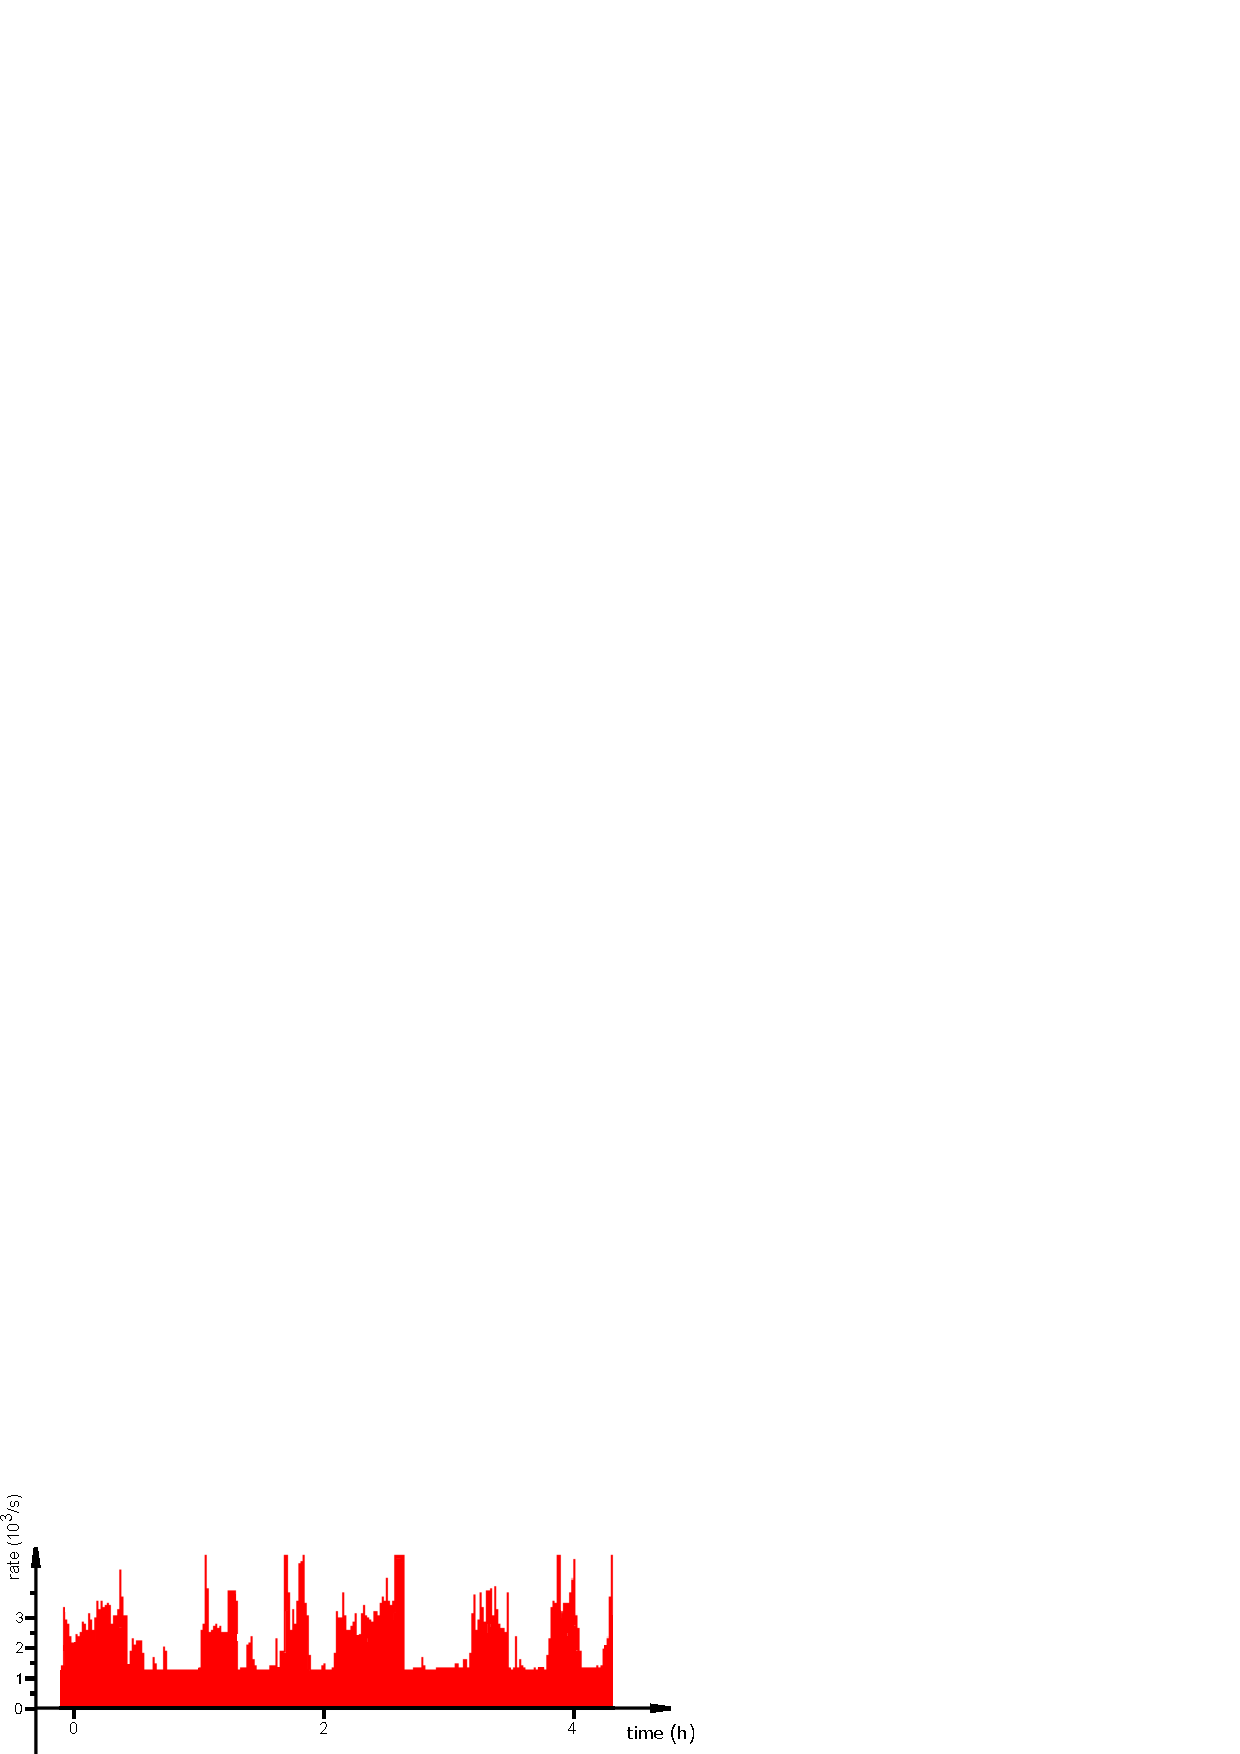
\includegraphics[width=0.9\textwidth]{graphics/setup/Noise_Rate_Problem_cutout_m.png}
   \caption[Muon modules' rate: noise problems]{Rate progression over the course of hours. The cumulative rate of all panels shows stron increases in certain intervals. In between it seems stable at around \SI{1200}{\per\second}. Note that this data was taken before adaption of the acceleration voltages (see later in this section) which is why the single module shows rates of \SI{150}{\per\second} only. }
  \end{figure}
  
  \begin{figure}
   \centering
   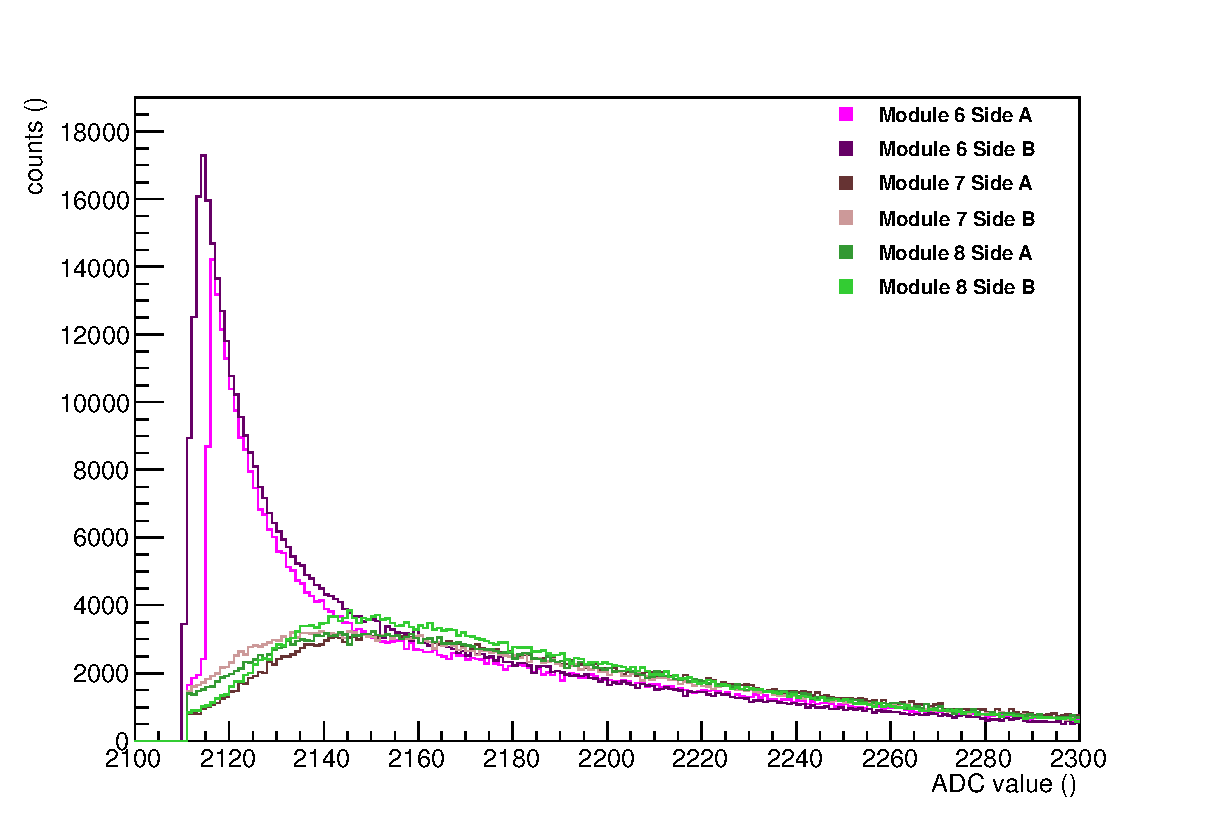
\includegraphics[width=0.9\textwidth]{graphics/setup/histogramNoise.eps}
   \caption[Six channel energy histogram with noise]{Energy histogram of six channels, i.e. modules 6 through 8 .Displayed are counts over ADC-Value. Both sides of module 6 show a lot of noise at the low energy end of the histogram while the cards other channels are developing clear Landau peaks.}
  \end{figure}
  
  As a countermeasure, in cooperation with Sascha Wuestling, potential equalization by connecting the modules to the trough below the main spectrometer has been established. This showed to prevent the peaking so the issue seems to be resolved. Now, gains, thresholds and acceleration voltages could be set (figure \ref{fig:allPeaksBefore}).
  
	At first, the acceleration voltages were kept low to limit the signal peaks' heights to around \SI{2}{\volt}. Carefully setting the mentioned parameters, one achieved the well aligned distributions from figure \ref{fig:allPeaksBefore}. A problem remaining at the time though was that the electronic noise set in pretty close to the peak position, only slightly shifted to lower energies. This made it not only very difficult to find suitable settings, but also meant that thresholds hat to be set close to the peak bin loosing low energy events in the process (see figure \ref{fig:allPeaksBefore}). This showed in rates of around \SI{150}{\hertz} that did not compare too well to literature values. The high energy region though was well fittable with landau distributions.\\
	\begin{figure}
		\centering
		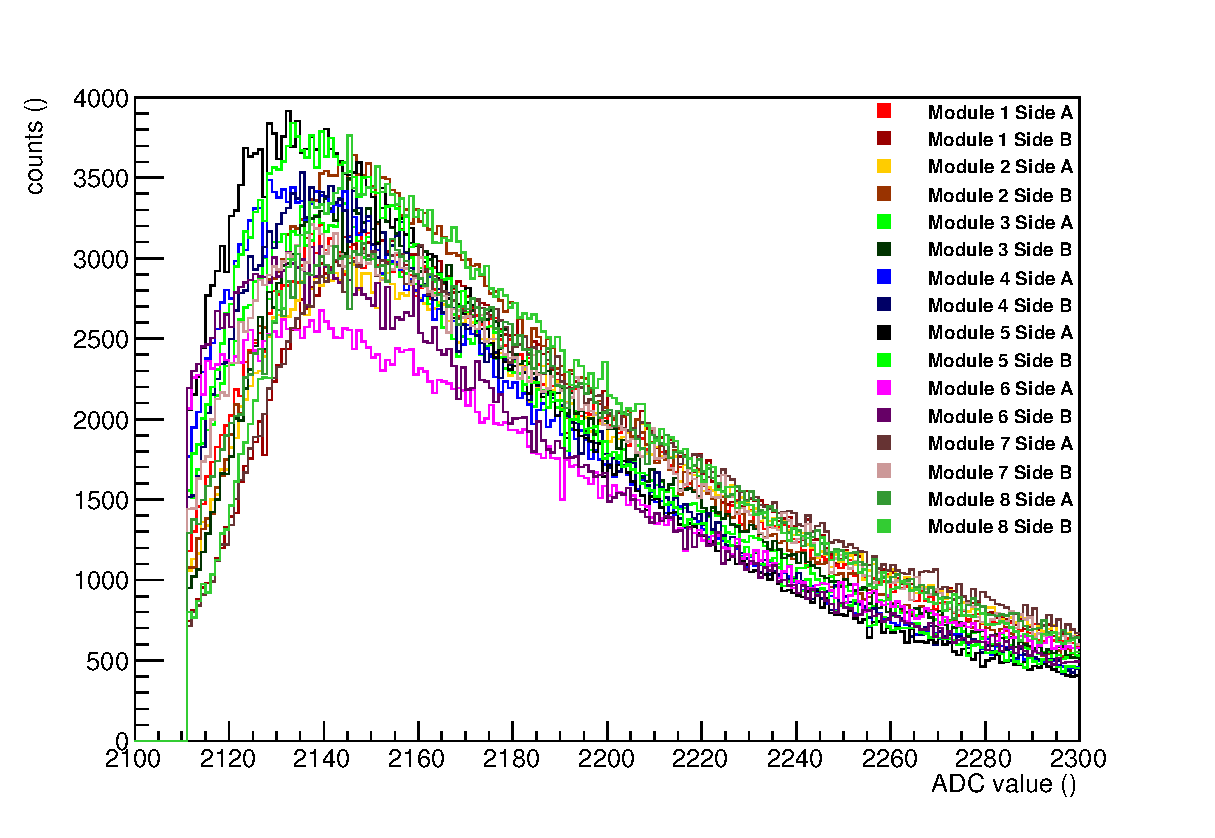
\includegraphics[width = 0.9 \textwidth]{graphics/setup/LandauPeaksRun660_old.eps}
		\caption[Landau peak \SI{1200}{\volt} acceleration voltage]{The landau peak at acceleration voltages about \SI{1200}{\volt}. All channels show comparable width and height. Note that the thresholds had to be set pretty close to the peak position as noise was a huge issue under the conditions of too low acceleration voltages.}
		\label{fig:allPeaksBefore}
	\end{figure}\\
	Later in the commissioning process, it got clear from the handbooks that the photomultiplier tubes had to be operated at acceleration voltages of \SI{1.5}{\kilo\volt} and above. 
	This was found as the detection efficiencies \ref{ch:Analysis:sec:Module Efficiency} for the modules were not as high as expected, assuming that the acceleration voltages set lower than denoted in the user manual leads to loss of data in the low energy range.
	Consequently, the acceleration voltages were raised to \SI{1.5}{\kilo\volt} except for two channels, those of modules 2B and 6A, that were even ramped to \SI{1.6}{\kilo\volt} on account of showing lower overall rates.
	Most of the tubes were limited to this minimal voltage to keep the signals' height as small as possible protecting the DAQ from taking damage. Following this procedure, the tubes seemed much more stable and rates more comparable, as all the gains and thresholds could now be set to the same values of \SI{0}{} \todo{enter thresh value} and \SI{20}{} respectively, while still showing well aligned peak positions \ref{fig:allPeaksAfter}. This is a huge advance to before when gains varied by factors almost up to four as it reduces potential non-linearities in amplification. Also, gains are left at lower values to begin with, leaving a larger part of the all in all amplification to the photomultiplier tubes known for their linear behavior and relatively low noise.
  
	\begin{figure}
		\centering
		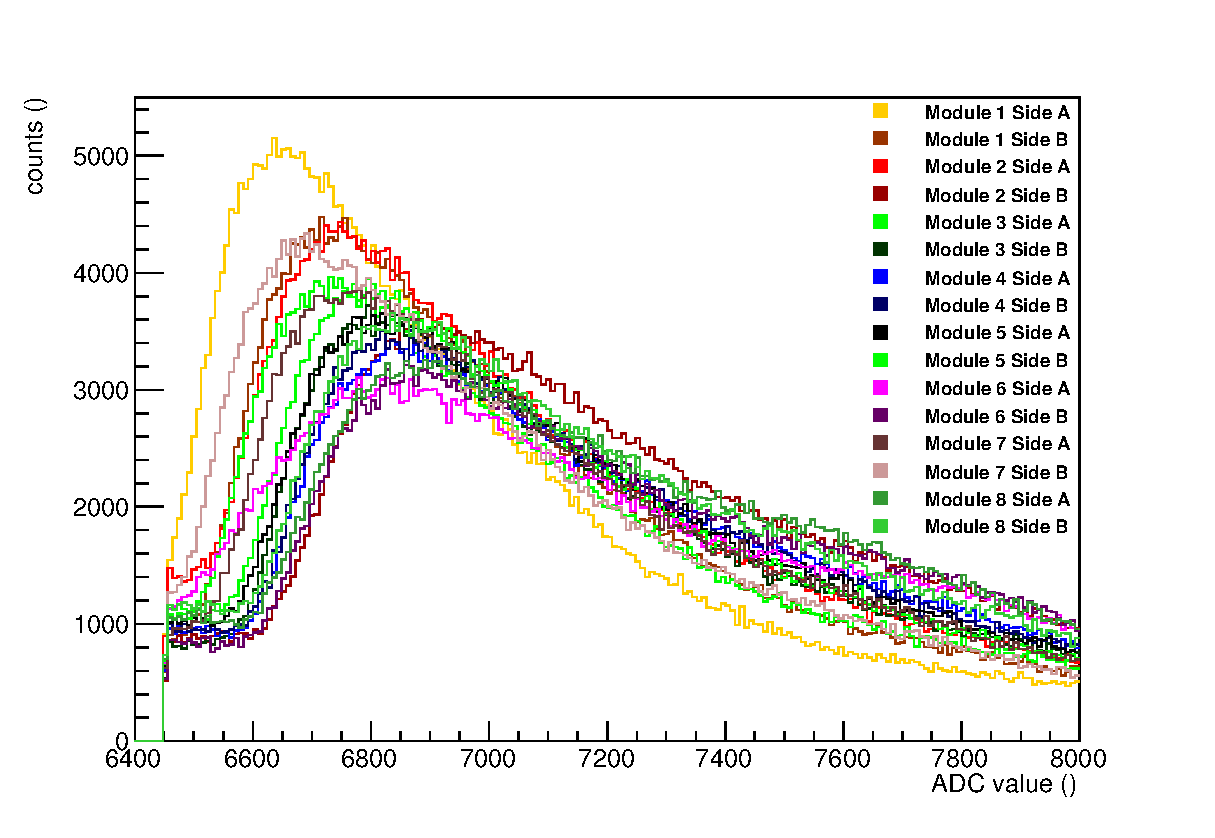
\includegraphics[width = 0.9 \textwidth]{graphics/setup/LandauPeaksRun1097_new.eps}
		\caption[Landau peak \SI{1500}{\volt} acceleration voltage]{Landau peaks after raising acceleration voltages to \SI{1.5}{\kilo\volt} (\SI{1.6}{\kilo\volt} for 2B and 6B). Note that this pattern was achieved solely by raising two module's side's acceleration voltages to \SI{1.6}{\kilo\volt} leaving gains and thresholds at the same low level for all channels. }
		\label{fig:allPeaksAfter}
	\end{figure}
	
	

